\documentclass[12pt,a4paper]{report}
\usepackage{geometry}
\usepackage{hyperref}
\hypersetup{
  colorlinks=true,
  linkcolor=black,
  citecolor=black,
  filecolor=black,
  urlcolor=black
}
\usepackage{graphicx}
\usepackage{booktabs}
\usepackage{array}
\usepackage{caption}
\usepackage{float}
\usepackage{amsmath}
\usepackage{cite}
\usepackage[table]{xcolor}
\usepackage{setspace}
\usepackage{fontspec}
\usepackage{etoolbox}
\usepackage{titlesec}

\geometry{top=2.2cm,bottom=1in,left=1in,right=1in}
\setmainfont{Trebuchet MS}
\onehalfspacing
\renewcommand{\contentsname}{Table of Contents}

\titleformat{\chapter}[display]
  {\normalfont\huge\bfseries}{}{0pt}{\centering}
\titlespacing{\chapter}{0pt}{-40pt}{10pt}

\makeatletter
\patchcmd{\@makechapterhead}{\vspace*{50\p@}}{\vspace*{0pt}}{}{}
\patchcmd{\@makeschapterhead}{\vspace*{50\p@}}{\vspace*{0pt}}{}{}
\makeatother
\titlespacing\section{0pt}{5pt}{5pt}

\begin{document}

% ---------------- Title Page ---------------- %
\begin{titlepage}
    \centering
    
\includegraphics[width=0.9\textwidth]{img/UCU.png}\\[1cm]
    {\Huge\bfseries Smart Fish Pond Management System: An IoT-Based Approach for Sustainable Aquaculture in Uganda \par}
    \vspace{1.5cm}
    {\LARGE\itshape\textbf{Project Proposal}\par}
    \vspace{1.0cm}
    

    {\Large\itshape\textbf{Submitted By:}\par}
    \vspace{0.8cm}

    % ---- group name here ---- %
    {\Large\textbf{Group Alpha}}
    \vspace{0.5cm}

    \renewcommand{\arraystretch}{1.3}
    \rowcolors{2}{gray!10}{white}
    \begin{tabular}{|p{5cm}|p{3.5cm}|p{3.5cm}|}
        \hline
        \rowcolor{gray!25}\textbf{Name} & \textbf{Registration No.} & \textbf{Access No.} \\
        \hline
        Ezamamti Ronald Austine & S23B23-018 & B24252 \\
        \hline
        Kisa Emmanuel  & S23B23/028 & B24259\\
        \hline
        Tendo Calvin & S23B23/013 & B24247\\
        \hline
    \end{tabular}

\end{titlepage}

% ---------------- Table of Contents ---------------- %
\tableofcontents
\clearpage

% ---------------- Chapter One ---------------- %
\chapter{Chapter One: Introduction}
\section{Background}
Uganda ranks among Africa’s leading fish-producing nations, with Lake Victoria providing the majority of wild-caught Nile perch and tilapia. However, overfishing, pollution, and unregulated practices have severely depleted natural fish stocks. The Nile perch, which previously generated the highest export revenues, is no longer sustainably exploitable. Between 2023 and 2024, Uganda’s fish export volumes declined by 27.8\% and revenues by 21.9\%~\cite{DailyMonitor2025}, signaling a need to diversify production sources.

To address this gap, aquaculture particularly pond farming of Nile tilapia (\textit{Oreochromis niloticus}) and African catfish (\textit{Clarias gariepinus}), has emerged as a key growth area~\cite{aanyu2020potential}. These species are resilient, widely accepted in both local and regional markets, and suitable for controlled pond systems. However, aquaculture productivity remains below potential due to inadequate water quality management, limited technical knowledge, and reliance on manual monitoring methods~\cite{tumwesigye2022effect}. 

National policy frameworks such as Uganda’s Vision 2040 and the Fourth National Development Plan (NDP IV) emphasize agro-industrialization and ICT-driven modernization of agriculture. Within this framework, the integration of digital and embedded system technologies into aquaculture offers a pathway toward sustainable fish production, reduced post-harvest losses, and enhanced export competitiveness.


\section{Problem Statement}
Over the past five years, Uganda has faced recurrent fish mortality events caused by deteriorating pond water quality and poor management practices. From 2020 to 2025, reports and studies have consistently linked these events to oxygen depletion, eutrophication, and inadequate monitoring systems. 

In 2020, experts warned that the rapid expansion of cage fish farming in Lake Victoria was contributing to localized water contamination. In January 2021, the National Environment Management Authority (NEMA) attributed widespread fish deaths to low dissolved oxygen, worsened by decaying aquatic vegetation and pollution. A 2022 study revealed that more than 80\% of pond farmers in the Rwenzori region lacked sufficient knowledge of water quality management, leading to disease outbreaks and poor yields~\cite{tumwesigye2022effect}. Further incidents in 2023 and 2024 on Lakes Kyoga and Victoria underscored systemic weaknesses in pond monitoring, prompting the government to launch the SWAQ-Uganda initiative.

By 2024, water pollution had become a national crisis, aggravated by industrial waste, agricultural runoff, and sewage. \newpage \noindent A 2025 study reported increasing parasitic infections in tilapia and catfish associated with deteriorating water quality~\cite{mramba2023pond}. Meanwhile, fish export revenues declined by 21.9\%, from UGX 514.5 billion in 2023 to UGX 395.7 billion in 2024~\cite{DailyMonitor2025}. 

Existing imported water monitoring systems remain expensive, technically complex, and unsuitable for smallholder aquaculture. There is therefore an urgent need for a low-cost, solar-powered, and IoT-enabled solution capable of continuously monitoring water quality and automating corrective actions to sustain fish health and enhance productivity in Uganda’s aquaculture sector.


\section{Research Questions and Objectives}
\subsection{Research Questions}
The study is guided by the following questions:
\begin{enumerate}
    \item What are the major water quality parameters affecting tilapia and catfish survival in Ugandan fish ponds?
    \item How can IoT-based systems be used to monitor and automate pond management efficiently?
    \item What is the impact of real-time monitoring on reducing mortality and improving aquaculture yields?
    \item How can a locally built system be made affordable and sustainable for small-scale fish farmers?
\end{enumerate}

\subsection{Research Objectives}
\textbf{General Objective:}  
To design and prototype an IoT-based Smart Fish Pond Management System that supports sustainable aquaculture practices in Uganda.
\\

\noindent \textbf{Specific Objectives:}
\begin{itemize}
    \item To design a real-time monitoring system for pond water quality parameters (DO, pH, turbidity, ammonia, temperature, and water level).
    \item To automate corrective actions such as aeration and pumping using embedded control systems.
    \item To develop a GSM and mobile-based notification system for real-time farmer alerts.
    \item To evaluate the effectiveness and cost-efficiency of the proposed system under field conditions.
\end{itemize}

\section{Justification for the Study}
The project aligns with Uganda’s Vision 2040 and the National Development Plan IV (2025–2030), which emphasize ICT integration and agro-industrialization to enhance productivity and sustainability.  

\textbf{Technologically}, integrating IoT-based sensors with embedded systems enables continuous monitoring of pond conditions, reducing reliance on manual inspection and enhancing precision in water quality management~\cite{prapti2022internet}.  

\textbf{Economically}, the system minimizes fish mortality and operational losses, improving yields and profitability for smallholder farmers while contributing to the country’s aquaculture export recovery~\cite{byabasaija2025unlocking}.  

\textbf{Environmentally}, the solar-powered design promotes clean energy use and responsible water management, addressing SDG 6 (Clean Water and Sanitation) and SDG 13 (Climate Action).  

\textbf{Socially}, improving aquaculture sustainability supports rural employment, nutrition, and food security, in line with SDG 2 (Zero Hunger) and SDG 9 (Industry, Innovation and Infrastructure).
 

\section{Conclusion}
This study proposes a Smart Fish Pond Management System to tackle Uganda’s aquaculture challenges using an affordable, sustainable, and locally maintainable IoT-based solution. The system will help reduce fish mortality, improve yields, and empower farmers with actionable data for better decision-making. It is anticipated that the prototype will demonstrate measurable improvements in pond water quality management and establish a foundation for future integration of advanced analytics and computer vision technologies in aquaculture.

% ---------------- References ---------------- %
\renewcommand{\bibname}{References}
\addcontentsline{toc}{chapter}{References}
\bibliographystyle{IEEEtran}
\bibliography{SmartFish_References}

% ---------------- Appendix ---------------- %
\appendix
\chapter*{Appendix}
\addcontentsline{toc}{chapter}{Appendix}

\begin{figure}[H]
    \centering
    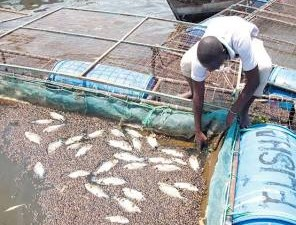
\includegraphics[width=0.5\textwidth]{img/low level.jpg}
    \caption{Low dissolved oxygen conditions in aquaculture ponds, a leading cause of fish mortality.}
    \label{fig:oxygen}
\end{figure}

\begin{figure}[H]
    \centering
    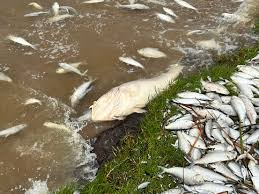
\includegraphics[width=0.5\textwidth]{img/dead fish.jpg}
    \caption{Mass fish mortality event in Uganda linked to poor water quality management and pollution.}
    \label{fig:deadfish}
\end{figure}

\begin{figure}[H]
    \centering
    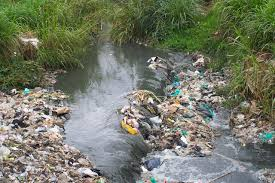
\includegraphics[width=0.5\textwidth]{img/waste.jpg}
    \caption{Waste accumulation and turbidity in pond water, increasing ammonia levels and stressing fish.}
    \label{fig:waste}
\end{figure}

\end{document}
